\section{Évaluation}
\begin{frame}
\frametitle{Évaluation}
\begin{itemize}
 \item Performance en terme de temps de vie de batterie ?
 \item Temps de réponse ?
 \item Impact de l'encapsulation TCP/IP ?
\end{itemize}
\vspace{5mm}
Dans les figures qui suivront,
\begin{itemize}
 \item (WS): Paquet envoyé avec une encapsulation TCP/IP %WS comme web service
 \item (barebone): Un paquet 802.15.4 sans header supplémentaire.
\end{itemize}
\end{frame}

\subsection{Consommation d'énergie}
\begin{frame}
 \frametitle{Coûts énergétiques}
 Mesure du temps de vie de batterie pour des payload allant de 1 à 80 octets.\\
 $\Rightarrow$ Suffisant pour les payload transmis lors du prototypage, utilisant le XML optimisé.\\
 Pour les paquets WS, le payload est encapsulé avec un header HTTP 1.1 pour un message request.
 \begin{block}{Remarque}
  Lorsque le payload dépasse 53 octets, il devient trop volumineux pour être envoyé en un seul paquet si on utilise une encapsulation TCP/IP et HTTP~1.1.
 \end{block}
\end{frame}

\def \radiosca {0.4}
\begin{frame}
 \frametitle{Temps de vie en fonction du payload}
 \framesubtitle{Radio éteinte entre les transferts TCP}
 \begin{figure}
  \centering
  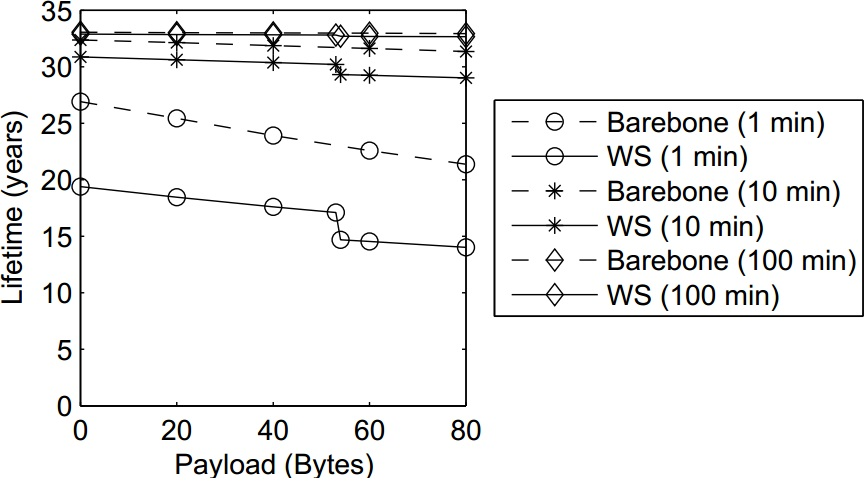
\includegraphics[scale=\radiosca]{figures/radiooff.jpg}
  \caption{Radio éteinte entre les transferts}
 \end{figure} 
\end{frame}

\begin{frame}
 \frametitle{Temps de vie en fonction du payload}
 \framesubtitle{Radio active pendant tout le transfert TCP}
 \begin{figure}
  \centering
  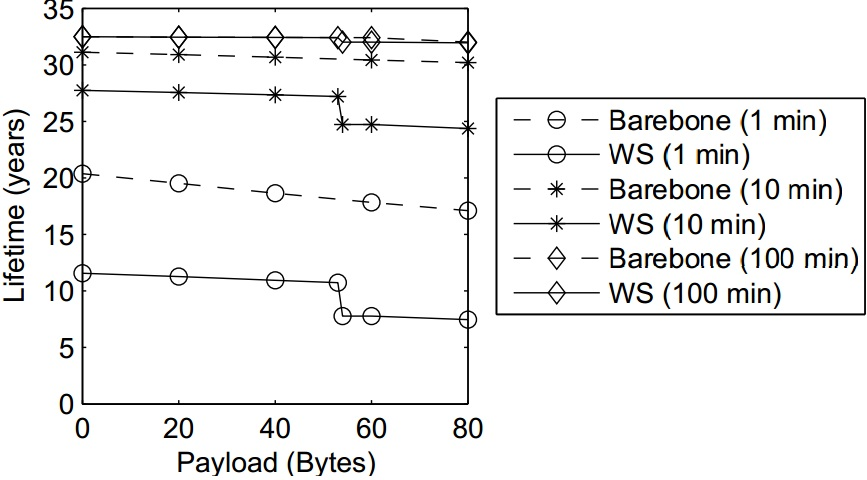
\includegraphics[scale=\radiosca]{figures/radioon.jpg}
  \caption{Radio allumée pendant toute la transmission}
 \end{figure} 
\end{frame}

%{Temps de vie en fonction du payload}{Observations} Oralement
 %Pour des messages inférieur à 53 octets, la taille a très peu d'impact sur le temps de vie
 %(réduction de 4,74\% pour des messages de 40 octets si radio éteinte entre les transferts, 10,85\% sinon).
 %C'est surtout la fréquence des messages qui réduit le temps de vie. Mais la plupart des applications ont une période moyenne entre 10 et 100 minutes.\\
 %En excluant les messages de période 1 minute, on observe donc que L'impact de l'overhead est négligeable}.
 %De plus, dans la réalité, des pertes de paquets et retransmissions auront lieu.Les paquets sans header ne sont donc pas envisageables.

\subsection{Temps de réponse}
\begin{frame}
 \frametitle{Temps de réponse}
 Mesure le temps entre l'envoi du paquet et la fin de son traitement dans le capteur.
 %(Lampe qui s'allume à distance).
 \begin{figure}
  \centering
  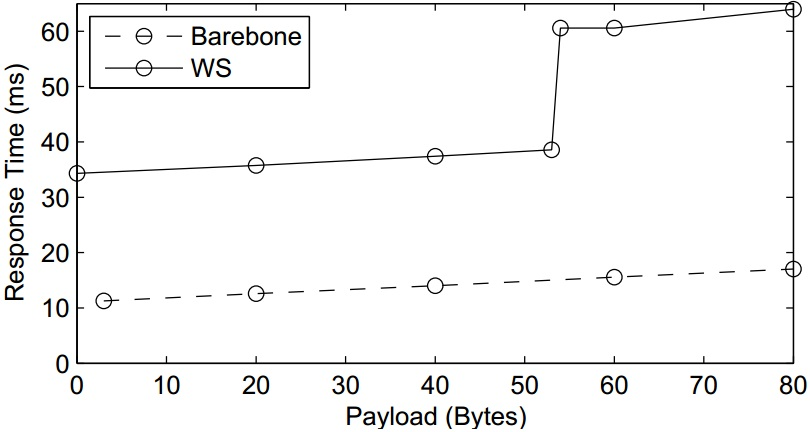
\includegraphics[scale=0.35]{figures/treponse.jpg}
  \caption{Temps de réponse}
 \end{figure} 
\end{frame}
 
%{Temps de réponse}{Observations} Oralement
 %Même envoyé en 2 paquets, le temps de réponse est toujours de quelques dizaines de millisecondes.
 %Ce qui est bien suffisamment court pour l'application qu'ils vont en faire.
 %Ici, TCP envoie un message ACK après chaque réception de paquet. ->Augmentation de latence lorsque le message est envoyé en 2 paquets.\\
 %Mais nous pouvons réduire cette augmentation:
%  \item Envoi de plusieurs paquets sans attendre un ACK entre chaque paquets envoyés.
%  \item Système de fragmentation/défragmentation sur la couche lien.
